\documentclass[a4paper,12pt]{article}
\usepackage[utf8]{inputenc}
\usepackage[serbian]{babel}
\usepackage{amsmath, amssymb}
\usepackage{graphicx}
\usepackage{booktabs}
\usepackage{float}
\usepackage{hyperref}
\usepackage{tabularx}
\usepackage{siunitx} 
\sisetup{group-separator = {\,}, group-minimum-digits = 4} 


\title{Višestruka regresija za predikciju cijene automobila u Srbiji}
\author{Teodor Vidaković}
\date{Jul 2025}

\begin{document}
\maketitle

\section{Eksplorativna analiza podataka}

Dataset sadrži informacije o oglasima polovnih automobila u Srbiji. Skup podataka ima ukupno 1756 primjera i 10 kolona, pri čemu ne postoje nedostajuće vrednosti. Korišćene kolone uključuju: \texttt{Marka}, \texttt{Grad}, \texttt{Godina proizvodnje}, \texttt{Karoserija}, \texttt{Gorivo}, \texttt{Zapremina motora}, \texttt{Kilometraža}, \texttt{Konjske snage}, \texttt{Menjač} i ciljnu promenljivu \texttt{Cena}.

\subsection{Osnovne statistike}

Nakon uklanjanja duplikata, ostaje 1353 validnih zapisa. Osnovne statistike za numeričke promjenljive prikazane su u Tabeli 1.

\begin{table}[H]
\centering
\caption{Osnovne statistike numeričkih promenljivih}
\label{tab:statistika}
\begin{tabularx}{\textwidth}{l *{6}{>{\raggedleft\arraybackslash}X}}
\toprule
\textbf{Atribut} & \textbf{Min} & \textbf{(25\%)} & \textbf{(50\%)} & \textbf{(75\%)} & \textbf{Max} & \textbf{Srednja} \\
\midrule
Cijena [EUR] & \num{1000} & \num{3000} & \num{5900} & \num{13500} & \num{999000} & \num{45027} \\
Godina proizvodnje & 1894 & 2006 & 2010 & 2015 & 2025 & 2010 \\
Zapremina motora [cm$^3$] & \num{163} & \num{1398} & \num{1600} & \num{1984} & \num{5461} & \num{1742.6} \\
Kilometraža [km] & \num{1000} & \num{165563} & \num{209000} & \num{256000} & \num{552000} & \num{206512} \\
Konjske snage & \num{45} & \num{92} & \num{116} & \num{150} & \num{620} & \num{129.5} \\
\bottomrule
\end{tabularx}
\end{table}

Vidimo da su cijene veoma varijabilne, pri čemu se maksimalna cijena kreće i do 999\,000 EUR, što ukazuje na prisustvo outlier-a. Većina automobila ima pređeno između 150\,000 i 300\,000 kilometara.

\subsection{Vizuelizacije}

U cilju grafičke analize podataka, korišćeni su sledeći prikazi:

\begin{itemize}
    \item \textbf{Histogram distribucije cijena} (Slika~\ref{fig:hist_cena})
    \item \textbf{Boxplot cijena} (Slika~\ref{fig:box_cena})
    \item \textbf{Korelaciona matrica numeričkih promenljivih} (Slika~\ref{fig:corr_matrix})
    \item \textbf{Scatterplot: Cijena vs. Starost vozila} (Slika~\ref{fig:starost_vs_cena})
\end{itemize}

\begin{figure}[H]
    \centering
    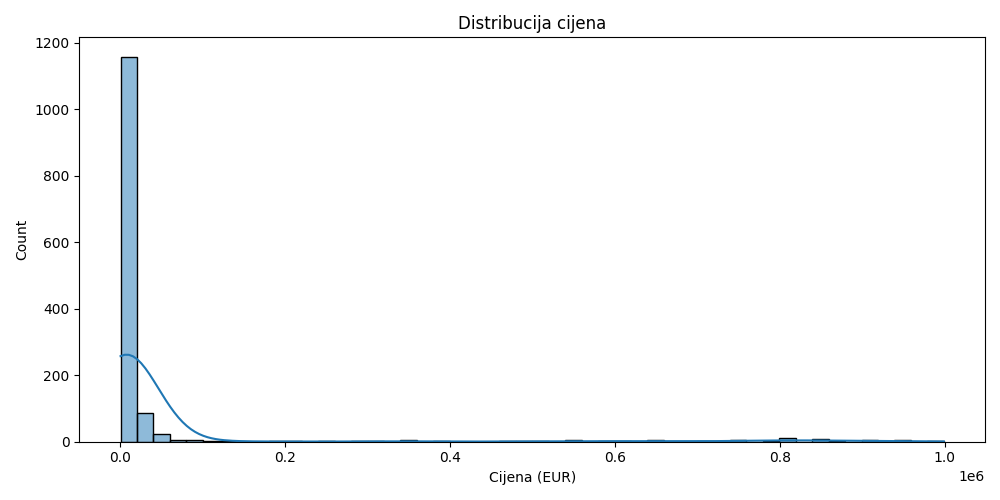
\includegraphics[width=0.7\textwidth]{hist_cena.png}
    \caption{Distribucija cijena automobila}
    \label{fig:hist_cena}
\end{figure}

\begin{figure}[H]
    \centering
    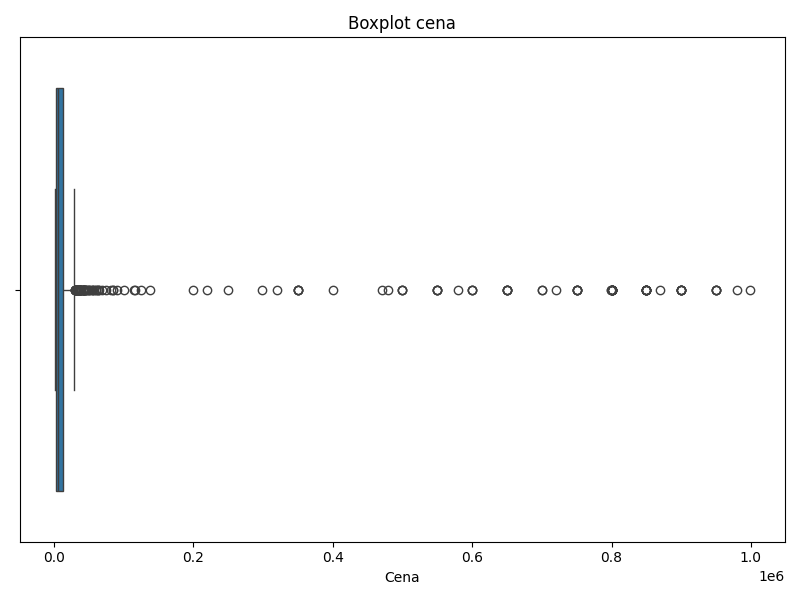
\includegraphics[width=0.7\textwidth]{box_cena.png}
    \caption{Boxplot cijena automobila}
    \label{fig:box_cena}
\end{figure}

\begin{figure}[H]
    \centering
    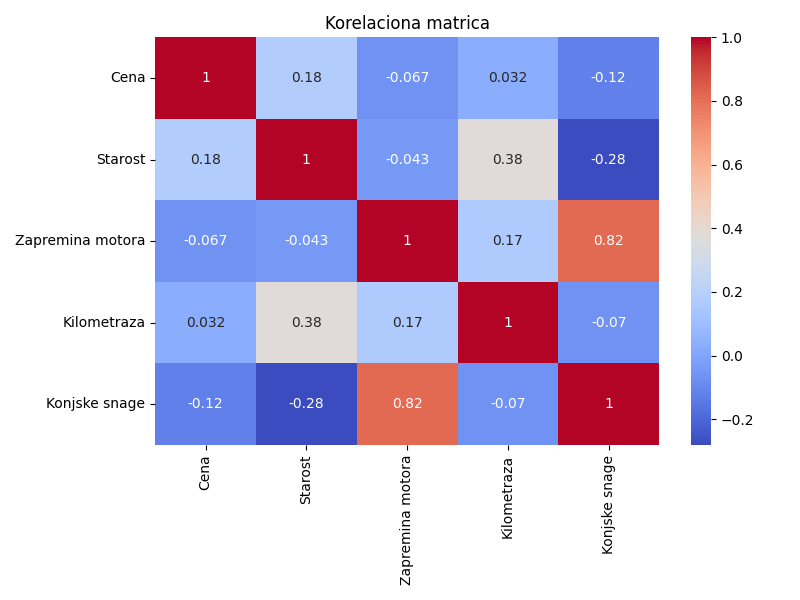
\includegraphics[width=0.65\textwidth]{corr_matrix.png}
    \caption{Korelaciona matrica numeričkih atributa}
    \label{fig:corr_matrix}
\end{figure}

\begin{figure}[H]
    \centering
    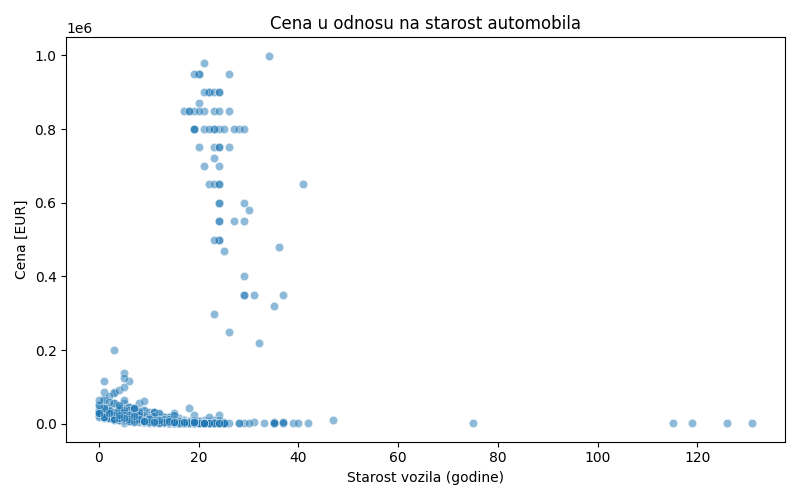
\includegraphics[width=0.7\textwidth]{scatter_starost_vs_cena.png}
    \caption{Raspodjela cijene u odnosu na starost vozila}
    \label{fig:starost_vs_cena}
\end{figure}

\subsection{Uočeni obrasci i anomalije}

Na osnovu vizuelne analize identifikovani su sledeći obrasci:

\begin{itemize}
    \item \textbf{Distribucija cijena je snažno asimetrična} (Slika~\ref{fig:hist_cena}) – većina vozila se prodaje ispod 20\,000 EUR, dok manji broj primjera sa cijenama od 100\,000+ EUR značajno odskače.
    
    \item \textbf{Prisustvo outlier-a potvrđeno je boxplot-om} (Slika~\ref{fig:box_cena}) – postoje brojni ekstremi koji narušavaju raspodjelu ciljne promjenljive i negativno utiču na RMSE.

    \item \textbf{Starost vozila i cijena imaju blago pozitivnu korelaciju} ($r = 0.18$), što je neočekivano. Međutim, scatterplot (Slika~\ref{fig:starost_vs_cena}) pokazuje da najskuplji automobili nisu novi, već stari — vjerovatno luksuzni, sportski ili kolekcionarski modeli. Većina novijih automobila (0–5 godina starosti) ima prosječnu ili nisku cenu, dok ekstremno visoke vrednosti dolaze od nekoliko skupocjenih vozila koja su stara 10+ godina. Ova nelinearna struktura dovodi do “lažne” pozitivne korelacije u linearnom smislu, iako bi se očekivala negativna veza između cijene i starosti.

    \item \textbf{Kilometraža ima vrlo slab odnos sa cijenom} ($r = 0.03$) – korisnici očigledno ne rangiraju ovaj faktor visoko pri određivanju cene.

    \item \textbf{Konjske snage i zapremina motora su visoko korelisani} ($r = 0.82$, Slika~\ref{fig:corr_matrix}) – što je i očekivano s obzirom na tehničku povezanost tih karakteristika.

    \item \textbf{Kategorijske promenljive su raznovrsne i zahtevaju kodiranje}:
    \begin{itemize}
        \item Marka: 44 vrednosti
        \item Grad: 236 različitih mesta (visoka disperzija)
        \item Karoserija i Gorivo: po 8 klasa
        \item Menjač: 2 klase (Manuelni i Automatski)
    \end{itemize}
\end{itemize}

\section{Preprocesiranje podataka}

Pre nego što je model treniran, podaci su prošli kroz preprocesiranje sa ciljem da se obezbjedi robusnost modela i smanji uticaj ekstremnih vrednosti.

\begin{itemize}
    \item \textbf{Filtriranje cijena} – Na osnovu prethodne analize, identifikovani su automobili sa ekstremno visokim cijenama (iznad 100\,000 EUR), koji značajno narušavaju distribuciju ciljne promenljive i utiču na RMSE. Umesto kvantilnog filtra, primenjena je jednostavna prag-filtracija: u dalji rad uključeni su samo primeri sa cijenom manjom ili jednakom \textbf{50\,000 EUR}. Time je uklonjen uticaj luksuznih i atipičnih vozila.

    \item \textbf{Uklanjanje duplikata} – Prije treniranja modela, duplirani oglasi su uklonjeni pomoću \texttt{drop\_duplicates()} metode.

    \item \textbf{Inženjering osobina} – Iz atributa \texttt{Godina proizvodnje} kreirana je nova numerička promjenljiva \texttt{Starost}, izračunata kao $2025 - \text{Godina proizvodnje}$. Ova osobina bolje opisuje uticaj vremena na gubitak vrijednosti vozila i zamjenjuje sirovu godinu.

    \item \textbf{Obrada numeričkih podataka} – Odabrane numeričke promjenljive su:
    \begin{itemize}
        \item \texttt{Starost}
        \item \texttt{Zapremina motora}
        \item \texttt{Kilometraža}
        \item \texttt{Konjske snage}
    \end{itemize}
    Kako bi model mogao da uoči nelinearne zavisnosti, na njih je primjenjena polinomska transformacija drugog stepena. Nakon toga, sve numeričke osobine su standardizovane (\texttt{StandardScaler}), što znači da je na njih primenjena z-score transformacija.

    \item \textbf{Obrada kategoričkih podataka} – Sledeće kolone su tretirane kao kategoričke:
    \begin{itemize}
        \item \texttt{Marka}, \texttt{Grad}, \texttt{Karoserija}, \texttt{Gorivo}, \texttt{Menjač}
    \end{itemize}
    Svaka od njih je kodirana tehnikom \textbf{One-Hot Encoding} kako bi se izbjegle greške pri predikciji na test skupu.

    \item \textbf{Log-transformacija ciljne promenljive} – Cijena automobila, kao ciljna promjenljiva, ima izraženu asimetričnu raspodjelu sa teškim desnim repom. Da bi se smanjio uticaj outlier-a i poboljšala stabilnost modela, izvršena je log-transformacija putem funkcije $\log(1 + y)$ pomoću \texttt{FunctionTransformer}. Predikcije su potom inverzno transformisane pomoću $\exp(y) - 1$.
	\begin{figure}[H]
	    \centering
	    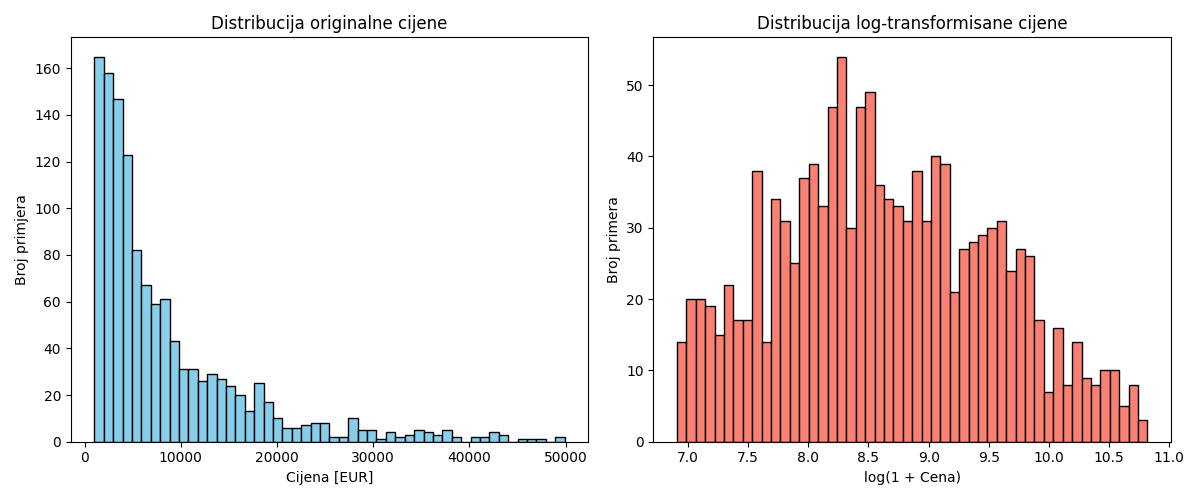
\includegraphics[width=\textwidth]{log_transformacija_cena.png}
	    \caption{Distribucija ciljne promenljive prije i poslije log-transformacije}
	    \label{fig:log_transform}
	\end{figure}
\end{itemize}

Nakon svih koraka, numeričke i kategoričke komponente objedinjene su pomoću \texttt{ColumnTransformer}. Transformacija ciljne promjenljive vršena je korišćenjem \texttt{TransformedTargetRegressor}, čime se obezbjeđuje konzistentna transformacija pri treniranju i predikciji.

\section{Podjela skupa podataka}

Za treniranje i evaluaciju modela korišćena su dva režima podjele podataka, u zavisnosti od konteksta pokretanja:

\begin{itemize}
    \item \textbf{Lokalna podjela podataka (lokalna evaluacija):} Kada se pokreće lokalno (npr. tokom eksperimentisanja), koristi se samo jedan skup podataka. U tom slučaju, podaci se dijele na trening i test skup pomoću funkcije \texttt{train\_test\_split} u odnosu 80:20. Da bi se očuvala reprezentativna distribucija ciljne promenljive, koristi se stratifikacija po cjenovnim opsezima.

    \item \textbf{Eksplicitna podela putem komandne linije:} Kada se skripta pokreće sa dva ulazna fajla (npr. \texttt{python model.py train.tsv test.tsv}), koristi se unaprijed pripremljeni trening i test skup, bez dodatne podjele unutar skripte. Ova varijanta se koristi za finalnu evaluaciju modela na test skupu koji nije korišćen u fazi treniranja.
\end{itemize}

Nakon što je trening skup definisan, primjenjena je \textbf{K-Fold unakrsna validacija} (\texttt{KFold}) sa brojem preklopa $k = 5$, uz opciju \texttt{shuffle=True} i fiksiran \texttt{random\_state=42} radi reproduktivnosti. Ova validacija ima dvostruku ulogu:

\begin{itemize}
    \item Unutar modela koristi se za automatsku selekciju optimalnog hiperparametra $\alpha$.
    \item Paralelno se koristi za procjenu performansi modela korišćenjem metrike RMSE, preko funkcije \texttt{cross\_val\_score}.
\end{itemize}

Ovaj pristup omogućava robusnu procjenu generalizacione sposobnosti modela bez curenja podataka iz test skupa. Nakon toga, model se trenira na cijelom trening skupu i koristi za evaluaciju na izdvojenom test skupu.

\section{Isprobani algoritmi}

Za zadatak višestruke regresije testirana su tri regularizovana linearna modela iz biblioteke \texttt{scikit-learn}: \texttt{LassoCV}, \texttt{RidgeCV} i \texttt{ElasticNetCV}. Svi modeli korišćeni su unutar istog pipeline-a.

\subsection{Podešavanje hiperparametara}

\begin{itemize}
    \item \textbf{LassoCV} bira optimalnu vrijednost regularizacionog parametra $\alpha$ iz logaritamski raspoređenog opsega od $10^{-4}$ do $10^{2}$ primjenom 5-fold unakrsne validacije.
    \item \textbf{RidgeCV} koristi isti opseg $\alpha$ vrijednosti i takođe primjenjuje 5-fold unakrsnu validaciju.
    \item \textbf{ElasticNetCV} osim $\alpha$ optimizuje i odnos između $L_1$ i $L_2$ regularizacije putem hiperparametra \texttt{l1\_ratio}, pri čemu su testirane vrednosti $\{0.1, 0.5, 0.9\}$.
\end{itemize}

\subsection{Rezultati}

Rezultati evaluacije prikazani su kroz metriku RMSE (na originalnoj skali, nakon inverzne log-transformacije), na osnovu 5-fold unakrsne validacije i konačnog lokalnog test skupa.

\begin{table}[H]
\centering
\caption{Uporedni rezultati modela sa 5-fold CV i lokalnim test skupom}
\label{tab:modeli}
\begin{tabularx}{\textwidth}{l >{\centering\arraybackslash}X >{\centering\arraybackslash}X >{\centering\arraybackslash}X}
\toprule
\textbf{Model} & \textbf{CV RMSE (mean ± std)} & \textbf{Test RMSE} & \textbf{Izabrani hiperparametri} \\
\midrule
LassoCV & $3045.09 \pm 250.22$ & $2638.25$ & $\alpha = 0.00107$ \\
RidgeCV & $3146.33 \pm 313.29$ & $2717.87$ & $\alpha = 4.03702$ \\
ElasticNetCV & $3049.26 \pm 269.87$ & $2657.75$ & $\alpha = 0.00187$, $l_1 = 0.50$ \\
\bottomrule
\end{tabularx}
\end{table}

\subsection{Diskusija}

Sva tri modela uspješno zadovoljavaju uslov RMSE < 6500 EUR na lokalnom  test skupu. Najbolje performanse ostvario je \textbf{LassoCV}, zahvaljujući sposobnosti selekcije relevantnih osobina putem $L_1$ regularizacije. Ridge je pokazao nešto lošije rezultate, dok je ElasticNet dao kompromis između prethodna dva pristupa.

\section{Odabrano rješenje}

Nakon eksperimentisanja sa različitim tehnikama preprocesiranja i modelima, kao najefikasnije rješenje izabran je model baziran na \texttt{LassoCV} regresiji sa sledećom konfiguracijom:

\begin{itemize}
    \item \textbf{Preprocesiranje podataka}:
    \begin{itemize}
        \item Numeričke promjenljive: proširene polinomskim osobinama drugog stepena (\texttt{PolynomialFeatures}) i zatim standardizovane pomoću Z-score standardizacije (\texttt{StandardScaler}).
        \item Kategoričke promenljive: kodirane One-Hot encoding-om sa ignorisanjem nepoznatih vrijednosti u test skupu.
        \item Inženjering osobina: uvedena nova numerička promjenljiva -- starost automobila (\texttt{Starost = 2025 - Godina proizvodnje}).
    \end{itemize}
    
    \item \textbf{Transformacija ciljne promjenljive}:
    \begin{itemize}
        \item Zbog izražene asimetrične distribucije cijena sa dugim desnim repom, izvršena je log-transformacija ciljne promjenljive pomoću $\log(1 + y)$, implementirana preko \texttt{FunctionTransformer}.
        \item Predikcije su inverzno transformisane sa $\exp(y) - 1$ kako bi se vratile na originalnu skalu.
    \end{itemize}
    
    \item \textbf{Model}:
    \begin{itemize}
        \item Regresor: \texttt{LassoCV} sa unakrsnom validacijom (\texttt{cv=5}) i automatskom selekcijom optimalnog hiperparametra $\alpha$ iz logaritamski raspoređenog skupa vrijednosti između $10^{-4}$ i $10^2$.
        \item Ovaj model vrši implicitnu selekciju osobina putem L1 regularizacije, što doprinosi smanjenju varijanse modela i otpornosti na overfitting.
    \end{itemize}
    
    \item \textbf{Validacija i performanse}:
    \begin{itemize}
        \item Tokom evaluacije korišćena je K-Fold unakrsna validacija (\texttt{KFold}, $k=5$, \texttt{shuffle=True}) i lokalni test skup dobijen stratifikovanom podjelom podataka.
        \item Postignuti rezultat na lokalnom test skupu:
        \[
        \text{Test RMSE} = \textbf{2638.25 EUR}
        \]
        što je značajno ispod zadatog praga od 6500 EUR.
        \item Izabrana vrijednost hiperparametra:
        \[
        \alpha = \textbf{0.00107}
        \]
    \end{itemize}
\end{itemize}

Ova konfiguracija predstavlja optimalan kompromis između predikcione tačnosti, robusnosti modela i interpretabilnosti, te je odabrana kao finalno rešenje.

\section*{Reference}

\begin{itemize}
    \item Pedregosa et al., \textit{Scikit-learn: Machine Learning in Python}, JMLR 2011.
    \item zvanična dokumentacija: \url{https://scikit-learn.org/stable/}
    \item Dataset: Oglasi automobila u Srbiji (projekat FTN, 2025)
\end{itemize}

\end{document}
